\documentclass[12pt]{article}

\usepackage{graphicx}
\usepackage{fixltx2e}
\usepackage{color,soul}
\usepackage{placeins}
\usepackage{amsmath,amsfonts,amsthm} 

% fonts
\usepackage[scaled=0.92]{helvet}   % set Helvetica as the sans-serif font
\renewcommand{\rmdefault}{ptm}     % set Times as the default text font

% dmb: not mandatory, but i recommend you use mtpro for math fonts.
% there is a free version called mtprolite.

% \usepackage[amssymbols,subscriptcorrection,slantedGreek,nofontinfo]{mtpro2}

\usepackage[T1]{fontenc}
\usepackage{amsmath}
\usepackage{amsfonts}

% page numbers
\usepackage{fancyhdr}
\fancypagestyle{newstyle}{
\fancyhf{} % clear all header and footer fields
\fancyfoot[R]{\vspace{0.1in} \small \thepage}
\renewcommand{\headrulewidth}{0pt}
\renewcommand{\footrulewidth}{0pt}}
\pagestyle{newstyle}

% geometry of the page
\usepackage[top=1in, bottom=1in, left=1in, right=1in]{geometry}

% paragraph spacing
\setlength{\parindent}{0pt}
\setlength{\parskip}{2ex plus 0.4ex minus 0.2ex}

% useful packages
\usepackage{natbib}
\usepackage{epsfig}
\usepackage{url}
\usepackage{bm}


\begin{document}

\begin{center}
  \Large \textbf{Applied Causality Final Report: The Meaning of Work and Productivity} \\
  \vspace{0.1in}
  \normalsize Natalie Carlson \\
  \today
\end{center}


\section{Introduction}

This course presented us with an exposure to causal inference dilemmas held by students across a variety of disciplines, the context of which may have at times been largely inscrutable to those of us coming from outside the area. I fear mine may have been no exception. I hoped, though, that the central question might prove universal: that is, what drives people to find their work to be meaningful, and does that sense of meaning in turn make them more productive workers. 

The context for my observational data comes from a 2012 survey, run at 571 microfinance branches nested within 19 organizations, across six states in India. At each branch, the branch manager and two loan officers were interviewed. The surveys were extensive, covering details on their activities breakdown, training, payment schemes, incentives, education and background, job enjoyment, and social measures, as well as details on the social service activities of the branch itself. The survey was intended to produce work on management practices and complementarities. The meaning-productivity relationship was something I noticed because it is a particular interest of mine.

The relationship in question I found striking: a clear, linear association between how meaningful the employees of a particular branch reported their work to be and the productivity of that branch. There is a great deal of literature in organizational behavior that suggests that employees who find meaning in their work will have higher levels of engagement, but no one had demonstrated a clear link to actual productivity. To be able to do so definitively would be of interest to both academics and practitioners.


\section{Previous Literature}

As previously mentioned, there is a large body of literature on meaning and the meaningfulness of work in the organizational behavior space. A perusal of Rosso et al.'s literature review (2010), though, shows that the vast majority of this work focuses on the antecedents of and the psychological processes behind the generation of meaning, rather than its impacts. To the extent that prior work is concerned with the effects of meaningfulness in work, it is usually focused on engagement. Indeed, the seminal work of Kahn (1990) on employee engagement places experienced meaningfulness among the three drivers of engagement, along with psychological safety and experienced availability.

In terms of quantitative evidence on meaning driving engagement, though, results are limited and mixed (Bailey \& Madden, 2017). Some of the most interesting work on meaningfulness in the workplace is qualitative in nature and derived from in-depth interviews. Pratt \& Ashforth (2003) emphasize that workplace meaningfulness is derived from community building, suggesting that two key elements are necessary for creating an organizational community: a family-like atmosphere, and a mission-driven focus with an emphasis on values. This values focus is echoed in Bailey and Madden's qualitative work on meaning (2016), in which they find that employees' sense of meaning appears to be a deeply personal and individual phenomenon, focused on their work's wider contribution to society. They also delve deep into the symmetric construct of meaninglessness, an event for which the most commonly cited cause was a conflict with the employee's personal value system.

The most closely related experimental evidence comes from an online experiment on prosocial incentives and productivity (Tonin \& Vlassopoulous 2015). In this experiment, online workers performing a simple piece-rate data entry task were given an additional incentive: a donation to a charitable organization would be made as a result of their work. They found that this incentive increased task productivity by 13 percent, and that the effect was larger for those who were predisposed to prosocial motivation (those who reported volunteering in their free time). 

The fact that individual preferences and value systems may moderate the relationship between meaningfulness and productivity will play heavily into this analysis. Particularly, the observational dataset comprises microfinance organizations with different ownership types and identities: NGOs; for-profit firms known as NBFCs; and a subset of organizations which began as NGOs but morphed at some point into a for-profit model (hereafter referred to as switchers). The nature of these organization types may attract different employees and breed different cultures. Battilana and Dorado (2010) describe microfinance institutions in general as hybrid organizations, combining both a "development logic" and a "banking logic". The switching companies in our sample, having been both non-profit and for-profit at different points in their life cycle, may fit this hybrid definition more than the others. 

\section{Observational Results and Causal Model}

\begin{align} 
\begin{split}
Y_i = \alpha_i + \delta M_i + \beta X_i + \epsilon_i
\end{split}					
\end{align}

\begin{align} 
\begin{split}
Y_i = \alpha_i + \delta_{NGO} M_i  [NGO=1]+ \delta_{NBFC} M_i  [NBFC=1] + \delta_{Switch} M_i  [Switch=1] \\
 +  \beta X_i + \epsilon_i
\end{split}					
\end{align}


-describe causal model and how it fits into literature
-equations for linear models
-summarize tables
-summarize changes in productivity var? 


\section{The Crux of the Causality Issue}

-discussion of reverse causality, difficulty in isolating effect
-description in terms of the do operator
-Gelman discussion of reverse vs forward causality

\section{Experimental Design}

-experiment in context of causal model

\section{Conclusion and Future Directions}

\section*{Appendix}

\begin{figure} [!h]
\centering
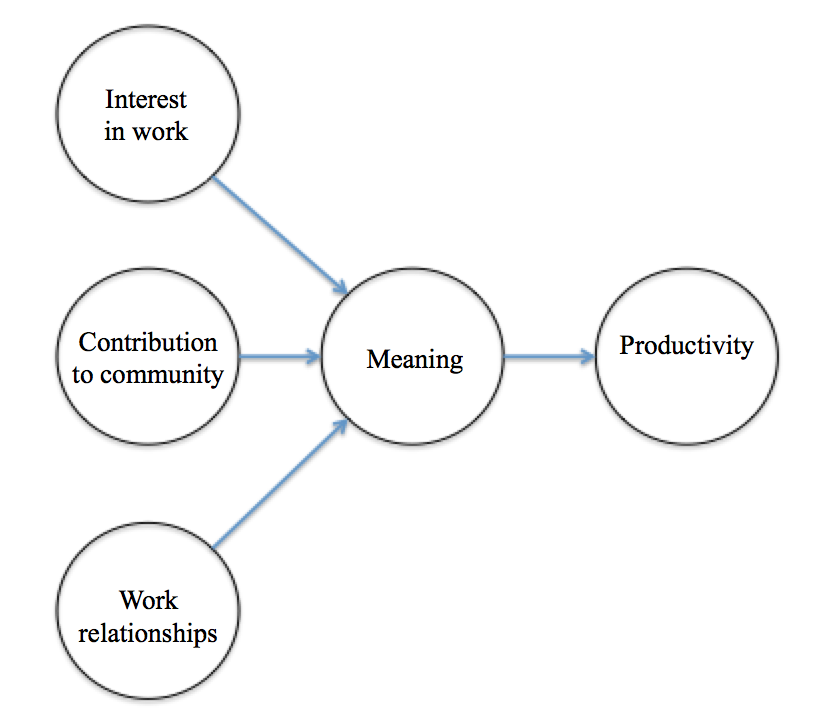
\includegraphics[scale=0.75]{causal_diagram}
\caption{Proposed causal graph}
\end{figure}

% Table created by stargazer v.5.2 by Marek Hlavac, Harvard University. E-mail: hlavac at fas.harvard.edu
\begin{table}[!htbp] \centering 
  \caption{Productivity Regressions} 
  \label{} 
\footnotesize 
\begin{tabular}{@{\extracolsep{5pt}}lcccc} 
\\[-1.8ex]\hline 
\hline \\[-1.8ex] 
 & \multicolumn{4}{c}{\textit{Dependent variable:}} \\ 
\cline{2-5} 
\\[-1.8ex] & \multicolumn{4}{c}{Productivity measure (standardized)} \\ 
\\[-1.8ex] & (1) & (2) & (3) & (4)\\ 
\hline \\[-1.8ex] 
 \textbf{`I sometimes feel my job is meaningless'} & \textbf{$-$0.14$^{**}$} & \textbf{$-$0.13$^{***}$} & \textbf{$-$0.09$^{**}$} &  \\ 
  & (0.06) & (0.05) & (0.04) &  \\ 
  `I sometimes feel my job is meaningless' x NGO &  &  &  & \textbf{$-$0.14$^{***}$} \\ 
  &  &  &  & (0.05) \\ 
  `I sometimes feel my job is meaningless' x NBFC &  &  &  & 0.01 \\ 
  &  &  &  & (0.03) \\ 
  `I sometimes feel my job is meaningless' x Switch &  &  &  & \textbf{$-$0.16$^{*}$} \\ 
  &  &  &  & (0.09) \\ 
  Always NGO &  & $-$0.42 & $-$0.01 & $-$0.09 \\ 
  &  & (0.32) & (0.02) & (0.26) \\ 
  Always NBFC &  & $-$0.13 & $-$0.04 & $-$0.54$^{**}$ \\ 
  &  & (0.25) & (0.04) & (0.27) \\ 
  Constant & 0.36$^{*}$ & 0.78$^{***}$ & 1.87$^{***}$ & 2.28$^{***}$ \\ 
  & (0.22) & (0.30) & (0.30) & (0.43) \\ 
 \hline \\[-1.8ex] 
Controls & No & Yes & Yes & Yes \\ 
State fixed effects & No & No & Yes & Yes \\ 
MFI fixed effects & No & No & Yes & Yes \\ 
\hline \\[-1.8ex] 
Observations & 423 & 396 & 396 & 396 \\ 
R$^{2}$ & 0.03 & 0.08 & 0.32 & 0.33 \\ 
\hline 
\hline \\[-1.8ex] 
\textit{Note: SEs clustered by MFI}  & \multicolumn{4}{r}{$^{*}$p$<$0.1; $^{**}$p$<$0.05; $^{***}$p$<$0.01} \\ 
\end{tabular} 
\end{table} 



% Table created by stargazer v.5.2 by Marek Hlavac, Harvard University. E-mail: hlavac at fas.harvard.edu
\begin{table}[!htbp] \centering 
  \caption{Drivers of Meaning} 
  \label{} 
\footnotesize 
\begin{tabular}{p{7cm}cccccc} 
\\[-1.8ex]\hline 
\hline \\[-1.8ex] 
 & \multicolumn{5}{c}{\textit{Dependent variable:}} \\ 
\cline{2-6} 
\\[-1.8ex] & \multicolumn{5}{c}{I sometimes feel my job is meaningless} \\ 
\\[-1.8ex] & (1) & (2) & (3) & (4) & (5)\\ 
\hline \\[-1.8ex] 
 \textbf{Took job because of interest in work} & \textbf{$-$0.10$^{***}$} &  &  & \textbf{$-$0.09$^{***}$} & \textbf{$-$0.09$^{***}$} \\ 
  & (0.03) &  &  & (0.03) & (0.02) \\ 
  \textbf{'Our company contributes positively to the community'} &  & \textbf{$-$0.28$^{***}$} &  & \textbf{$-$0.23$^{**}$} & \textbf{$-$0.24$^{**}$} \\ 
  &  & (0.10) &  & (0.10) & (0.10) \\ 
  \textbf{'I like the people I work with'} &  &  & \textbf{$-$0.24$^{**}$} & \textbf{$-$0.19$^{**}$} & \textbf{$-$0.21$^{**}$} \\ 
  &  &  & (0.09) & (0.10) & (0.09) \\ 
  BM total compensation (std) &  &  &  &  & 0.12 \\ 
  &  &  &  &  & (0.08) \\ 
  LO total compensation (std) &  &  &  &  & 0.06 \\ 
  &  &  &  &  & (0.10) \\ 
  Always NGO & 0.05 & $-$0.05 & $-$0.002 & 0.04 & 0.11 \\ 
  & (0.05) & (0.04) & (0.04) & (0.04) & (0.08) \\ 
  Always NBFC & 0.69$^{***}$ & 0.44$^{***}$ & 0.53$^{***}$ & 0.63$^{***}$ & 0.62$^{***}$ \\ 
  & (0.06) & (0.03) & (0.02) & (0.05) & (0.06) \\ 
  Constant & 1.87$^{***}$ & 3.11$^{***}$ & 2.70$^{***}$ & 4.46$^{***}$ & 4.67$^{***}$ \\ 
  & (0.37) & (0.81) & (0.53) & (0.82) & (0.89) \\ 
 \hline \\[-1.8ex] 
Controls & Yes & Yes & Yes & Yes & Yes \\ 
State fixed effects & Yes & Yes & Yes & Yes & Yes \\ 
MFI fixed effects & Yes & Yes & Yes & Yes & Yes \\ 
\hline \\[-1.8ex] 
Observations & 455 & 455 & 455 & 455 & 454 \\ 
R$^{2}$ & 0.20 & 0.19 & 0.17 & 0.23 & 0.24 \\ 
\hline 
\hline \\[-1.8ex] 
\textit{Note: SEs clustered by MFI}  & \multicolumn{5}{r}{$^{*}$p$<$0.1; $^{**}$p$<$0.05; $^{***}$p$<$0.01} \\ 
\end{tabular} 
\end{table} 




\end{document}
